\section{Convergence and Incentive Results}
\label{analysis}
In this section, we present the theoretic analysis for our incentive mechanism\footnote{Currently, our theoretical analysis is for the case that $m_i^t=M$. $m_i^t<M$ requires to replace the binomial distribution with the trinomial distribution when analyzing a key function involved in the proof in the supplementary file. The main idea of proof will be the same, and we will extend our proof in the future work.}. Our main results are as follows:
\begin{theorem}[One-Step IC]
\label{OSEqulibrium}
In any time step $t$, when $M\gg 1$, $(2\mathbb{P}_H)^{2(N-1)} \geq M$ and $a_t>\frac{c_H}{\mathbb{P}_H-0.5}$, reporting truthfully and exerting high efforts is the utility-maximizing strategy for any worker $i$ if the other workers all follow this strategy.
\end{theorem}
\begin{theorem}[Long-Term IC]
\label{RMNE}
Suppose the conditions in Proposition~\ref{OSEqulibrium} are satisfied and the learned $Q$-function approaches the real $Q(\hat{s},a)$. When
\begin{align}
&\eta M(N-1)\mathbb{P}_H \cdot G_{\mathcal{A}}> \frac{F(1)-F(1-\psi)}{1-\gamma}\label{Condition}\\
&\;\psi =(\tau_1\tau_2^{-1}+\tau_1^{-1}\tau_2)[4\mathbb{P}_H(1-\mathbb{P}_H)]^{\frac{N-1}{2}} \label{equation:psi}
\end{align}
always reporting truthfully and exerting high efforts is the utility-maximizing strategy for any worker $i$ in the long-term if the other workers all follow this strategy. Here, $G_{\mathcal{A}}=\min_{a,b\in\mathcal{A}, a\neq b}|a-b|$ denotes the minimal gap between two available values of the scaling factor.
\end{theorem}
In the following two subsections, we will provide the outline of the proofs of these two theorems. 
Note that, in addition to incentive compatiblity, our mechanism can also get rid of the undesired uninformative equlibrium that most peer prediction mechanisms have.
See Appendix G in the supplementary file for detailed discussion.
Besides, in our proof, if we omit the superscript $t$ in an equation, we mean that this equation holds for all time steps.
Besides, we employ the convention that $\bar{\mathbb{P}}=1-p$, $\hat{\mathbb{P}}=\max \{\mathbb{P}, \bar{\mathbb{P}}\}$ and $\mathbb{P}_0=\tau_1$.

%To prove Proposition~\ref{RMNE}, we need to analyze worker $i$'s effects on our reinforcement learning algorithm.
%If worker $i$ wishes to get higher payments in the long term, he/she must push our reinforcement learning algorithm to at least increase the scaling factor from $a$ to $b>a$ at a certian state $s$.
%In the $\epsilon$-greedy strategy used by our reinforcement learning algorithm, the random selection part is independent of worker $i$.
%Thus, worker $i$ must mislead the greedy part by letting $\tilde{Q}(s,a)\leq \tilde{Q}(s,b)$.
%In this proof, we will show that, under the condition defined in Equation~\ref{Condition}, there does not exist $b\in \mathcal{A}$ that can achieve this objective.
%In other words, our reinforcement learning algorithm will never increase the scaling factor to please a single worker.
%On the other hand, in any time step $t$, worker $i$ will loss some money if $p_i^t<p_H$.
%Thereby, the payment-maximizing strategy for worker $i$ is to report truthfully and exert high efforts in all time steps, which concludes Proposition~\ref{RMNE}.
% $\tilde{P}^t_i$ is calculated based on
%From our payment rule defined in Equation~\ref{equation:payment}, we can know that
%
%From our payment rule defined in Equation~\ref{equation:payment}, we can know that the payment-maximizing strategy for worker $i$ should be the one that maximizes $\tilde{\mathbb{P}}^t_i$ because $a^t$, $m^t_i$ and $b$ are all given in the beginning of step $t$.
%In this case, if $\tilde{P}^t_i\approx \mathbb{P}^t_i$ holds (Step 3), Theorem~\ref{OSEqulibrium} can be obtained straightforwardly.
%$\tilde{P}^t_i$ is calculated based on Equation~\ref{equation:p_infer}.
%If all the generated samples of the true labels in Equation~\ref{equation:p_infer} are correct, namely $\tilde{\mathcal{L}}^{(s)}(j)\equiv\mathcal{L}(j)$, $\tilde{P}^t_i\approx \mathbb{P}^t_i$ holds because of the law of large numbers.
%This observation motivates us to analyze the upper bound of the ration of wrong labels in the generated samples.
%
%%, and our proof, as our core contributions, provide some novel ideas about the IC analysis of machine learning algorithms.
%Here, we provide an overview about our proof at first.
% 
%
%The proof of Proposition~\ref{OSEqulibrium} relies on the convergence of our Bayesian inference algorithm, namely $\tilde{p}_i^t\rightarrow p_i^t$.
%To prove Proposition~\ref{RMNE}, we need to bound the effects of a single worker on our reinforcement learning algorithm.
%This analysis provides a novel tool to prevent self-interested agents from manipulating reinforcement learning algorithm.


%More specifically, in the right-hand side Equation~\ref{Condition},
%\begin{equation}
%\psi =2(\tau_1\tau_2^{-1}+\tau_1^{-1}\tau_2)[4p_H(1-p_H)]^{\frac{N-1}{2}}
%\end{equation}
%is the upper bound of the label accuracy increment brought by a single worker.
%Thus, the right-hand side Equation~\ref{Condition} indicates the upper bound of the long-term utility increment that a single worker can bring.
%On the other hand, $\zeta= M(N-1)p_H$ and ${\min}_{a,b\in\mathcal{A}}|a-b|$ denotes the minimal gap between two available values of the scaling factor $a^t$.
%Thus, the left-hand side of Equation~\ref{Condition} is actually the lower bound of the payment increment if our reinforcement adjustment algorithm increases the scaling factor.
%Thereby, if Equation~\ref{Condition} is satisfied, a single worker will always be unable to cause our reinforcement adjustment algorithm to change $a^t$.
%This property ensures always reporting truthfully and exerting high efforts to be a Nash equilibrium, and also prevents the clever manipulation that a worker scarifies short-term benefits for higher payments in the future.
%In the remaining parts of this section, we will provide the details of our proof.
%It is also worth noting that we prove over 10 lemmas as the foundation of our proof.
%Due to the space limitation, we put them all in the supplementary file.


\subsection{Proof for One-Step IC}
Recall that, Eqn.\ref{equaton:score} and \ref{equation:p_infer} together show that $\sum_j \textsf{sc}_i(j)\approx M\cdot \tilde{\mathbb{P}}_i$ holds when $M\gg 1$. Then, when $a_t>c_H/(\mathbb{P}_H-0.5)$, if $\tilde{\mathbb{P}}^t_i\approx \mathbb{P}^t_i$, worker $i$'s utility-maximizing strategy will be reporting truthfully and exerting high efforts.\footnote{$u_i^t\approx  M\cdot a_t\cdot (\tilde{\mathbb{P}}_i-0.5) + M\cdot b- M \cdot c_H\cdot \textsf{eft}^{t}_i$. See Appendix~F in the supplementary file for more detailed discussion. 
%From the later analysis, we can know $\tilde{\mathbb{P}}_i\approx \mathbb{P}_i$. When $\textsf{rpt}^{t}_i=1$, $\textsf{eft}^{t}_i =|\mathbb{P}_i-0.5|/(P_H-0.5)$. When $\textsf{rpt}^{t}_i<1$, higher $\textsf{eft}^{t}_i$ is needed to reach $\mathbb{P}_i$, which will lead to more costs. However, the payment will not increase. Thus, the utility of worker $i$ willl decrease.
}
Thus, we can conclude Theorem~\ref{OSEqulibrium} by proving the convergence of our Bayesian inference algorithm, i.e. proving $\tilde{\mathbb{P}}^t_i\approx \mathbb{P}^t_i$.
$\tilde{\mathbb{P}}^t_i$ is computed according to Eqn.~\ref{equation:p_infer}, and if most of the samples in our Bayesian inference arecorrect, namely $\tilde{\mathcal{L}}^{(s)}(j)\equiv\mathcal{L}(j)$, we can prove $\tilde{\mathbb{P}}^t_i\approx \mathbb{P}^t_i$ by leveraging the law of large numbers.
This observation motivates us to bound $|\tilde{\mathbb{P}}^t_i-\mathbb{P}^t_i|$ by calculating the upper bound of the ratio of wrong labels in the samples.
Thereby, we prove Theorem~\ref{OSEqulibrium} with the following two steps:
%\underline{\textbf{Step 1}:} Denote the labels generated by $N$ workers for task $j$ as vector $\bm{L}(j)$.
%The distribution of $\bm{L}(j)$ satisfies
%\begin{equation}
%\mathbb{P}_{\hat{\bm{\theta}}}[\bm{L}(j)] = {\sum}_{k=1}^{2}\tau_k{\prod}_{i=1}^{N}\mathbb{P}_i^{\delta_{ijk}}(1-\mathbb{P}_i)^{\delta_{ij(3-k)}}
%\end{equation}
%where $\hat{\bm{\theta}}=[\tau_1, \mathbb{P}_1,\ldots,\mathbb{P}_N]$ denotes all the parameters and $\delta_{ijk}=\mathbbm{1}(L_i(j)=k)$.
%Then, we can have
%\begin{lemma}
%\label{Denominator}
%When $M\rightarrow \infty$, 
%\begin{equation*}
%\mathbb{P}(\bm{L})\rightarrow C_{L}(M) \cdot {\prod}_{\bm{L}(j)} \left\{\mathbb{P}_{\hat{\bm{\theta}}}[\bm{L}(j)]\right\}^{M\cdot \mathbb{P}_{\hat{\bm{\theta}}}[\bm{L}(j)]}
%\end{equation*}
%where $C_{L}(M)$ denotes a constant that depends on $M$.
%\end{lemma}
%We defer the proof to the supplementary material.
%Our main idea is to connect $\mathbb{P}(\mathcal{L})$ with ${\prod}_{j=1}^{M}\mathbb{P}_{\hat{\bm{\theta}}}[\bm{L}(j)] $.

\underline{\textbf{Step 1}:} In this step, we aim to derive the upper bound of the ratio of wrong samples in our Bayesian inference algorithm.
To achieve this objective , we introduce $n$ and $m$ to denote the number of tasks of which the true label sample in Eqn.\ref{equation:p_infer} is correct ($\mathcal{L}^{(s)}(j)=\mathcal{L}(j)$) and wrong ($\mathcal{L}^{(s)}(j)\neq \mathcal{L}(j)$), respectively.
Then, we are able to prove the following lemma:
\begin{lemma}
\label{ConvBound}
When $M\gg 1$,
\begin{align}
\mathbb{E}[m/M]&\lesssim (1+e^{\delta})^{-1}(\varepsilon+e^{\delta})(1+\varepsilon)^{M-1}\label{equation:CB1}\\
\mathbb{E}[m/M]^2&\lesssim (1+e^{\delta})^{-1}(\varepsilon^2+e^{\delta})(1+\varepsilon)^{M-2}\label{equation:CB2}
\end{align}
where $\varepsilon^{-1}=\prod_{i=0}^{N}(2\hat{\mathbb{P}}_i)^{2}$, $\delta=O[\Delta\cdot \log(M)]$ and 
$$\Delta={\sum}_{i=1}^N[1(\mathbb{P}_i<0.5)-1(\mathbb{P}_i>0.5)].$$
\end{lemma}
We defer the detailed proof to the supplementary material. Our main idea is to introduce a set of counts for the collected labels at first.
More specifically, among the $n$ tasks of which the posterior true label is correct, $x_i$ and $y_i$ denote the number of tasks of which worker $i$'s label is correct and wrong, respectively.
Among the remaining $m$ tasks, $w_i$ and $z_i$ denote the number of tasks of which worker $i$'s label is correct and wrong, respectively.
Then, we calculate the approximation of $\mathbb{P}(m)$ based on the conditional probabilities $\mathbb{P}(x_i,y_i,w_i, z_i|m)$ and $\mathbb{P}(\mathcal{L}|\bm{L})$.
The upper bounds of $\mathbb{E}[m/M]$ and $\mathbb{E}[m/M]^2$ can be obtained by calculating the upper bounds of $\sum_{m}m \mathbb{P}(m)$ and $\sum_{m} m^2 \mathbb{P}(m)$.

\underline{\textbf{Step 2}:} In this step, we derive the upper bound of $|\tilde{\mathbb{P}}_i-\mathbb{P}_i|$ under the conditions of Theorem~\ref{OSEqulibrium}. Following the notations in Step 1, when $M\gg 1$, in Eqn.\ref{equation:p_infer}, we can have $\tilde{\mathbb{P}}_i\approx \mathbb{E}_{\mathcal{L}}(x_i+z_i)/M$, where $\mathbb{E}_{\mathcal{L}}$ denotes the expectation against $\mathbb{P}(\mathcal{L}|\bm{L})$. Meanwhile, according to the law of large numbers, $\mathbb{P}_i\approx (x_i+w_i)/M$. Thus, we can have
\begin{equation}
|\tilde{\mathbb{P}}_i-\mathbb{P}_i|\approx \mathbb{E}_{\mathcal{L}}|w_i-z_i|/M\leq \mathbb{E}_{\mathcal{L}}\left[m/M\right].
\end{equation}
If workers except for worker $i$ all report truthfully and exert high efforts, then $\Delta \leq -1$ in Theorem~\ref{ConvBound} because we require $N\geq 3$ in Section~\ref{PF}.
Thus, $e^{\delta}\approx 0$.
Since $2\hat{\mathbb{P}}_i\geq 1$, we have $\varepsilon^{-1}\geq (2\mathbb{P}_H)^{2(N-1)}$.
Hence, $\varepsilon\leq M^{-1}$ when $(2\mathbb{P}_H)^{2(N-1)} \geq M$.
Taking the above analysis into consideration, Eqn.\ref{equation:CB1} and \ref{equation:CB2} can be calculated as
\begin{equation}
\mathbb{E}\left[\frac{m}{M}\right]\lesssim \frac{C_{1}}{M\cdot C_2}\;\;, \;\;\mathbb{E}\left[\frac{m}{M}\right]^2\lesssim \frac{C_{1}}{M^2\cdot C_2^2}
\end{equation}
where $C_{1}=(1+M^{-1})^{M}\approx e$ and $C_{2}=1+M^{-1}\approx 1$.
Then, $m/M\approx 0$ because $\mathbb{E}[m/M]\approx 0$ and $\mathrm{Var}[m/M]=\mathbb{E}[m/M]^2-(\mathbb{E}[m/M])^2 \approx 0$.
In this case, $\tilde{\mathbb{P}}_i\approx \mathbb{P}_i$ and 
Thereby, if $a^t>c_H$, worker $i$ can only get the maximal utility when $\mathbb{P}_i=\mathbb{P}_H$, which concludes Theorem~\ref{OSEqulibrium}.

%Thus, $\mathbb{E}_{\mathcal{L},\bm{L}}\left[m/M\right]\lesssim x(1+x)^{M-1}$. Considering $2\hat{p}\geq 1$, we can know that $x\geq (2p_H)^{2(N-1)}$. Then, when $M\rightarrow \infty$ and $(2p_H)^{2(N-1)}>M$, we can have $(1+x)^{M-1}\rightarrow e$ and $x\rightarrow 0$. In this case, $\mathbb{E}_{\mathcal{L}}|\tilde{p}_i-p_i|\rightarrow 0$.
%Besides, we know that $p_i$ reaches the maximum only when worker $i$ report truthfully and exert high efforts.
%Thereby, in our mechanism, workers can only maximize their rewards by reporting truthfully and exerting high efforts, which concludes Proposition~\ref{OSEqulibrium}.
%for the simplicity of notation, we write $\mathbb{E}_{\mathcal{L},\bm{L}}[\frac{m}{M}]$ and $\mathbb{E}_{\mathcal{L},\bm{L}}[\frac{m}{M}]^2$ as $u$ and $v$, respectively.
%Recalling our mechanism defined in Definition~\ref{MechDef}, to analyze workers' expected rewards, we need to calculate the expectation of $\hat{p}_i$, $\hat{p}^2_0$ and $(1-\hat{p}_0)^2$ at first.
%According to Equation~\ref{p_infer}, we know $\hat{p}_i\approx \mathbb{E}_{\bm{L}}(x_i+z_i)/M$. Thus, the expectation of $\hat{p}_i$ satisfies
%\begin{equation}
%\mathbb{E}_{\mathcal{L}}\hat{p}_i\approx{\sum}_{m,x_i,z_i}\frac{x_i+z_i}{M}P(x_i|n)P(z_i|m)P(m)
%\end{equation}
%For a given $m$, $x_i\sim\mathrm{Bin}(n, p_i)$ and $z_i\sim\mathrm{Bin}(m, 1-p_i)$.
%Thus, we can calculate the expectation as $\mathbb{E}_{\mathcal{L}}\hat{p}_i = p_i\left(1-u\right)+(1-p_i)u$.
%Meanwhile, $\hat{p}^2_0$ satisfies
%\begin{equation}
%\mathbb{E}_{\mathcal{L}}\hat{p}^2_0\approx{\sum}_{m=0}^{M}\frac{\mathbb{E}x^2_0+2\mathbb{E}x_0\mathbb{E}z_0+\mathbb{E}z^2_0}{M^2}P(m)
%\end{equation}
%where the expectation of the square should satisfy $\mathbb{E}x^2_0=(\mathbb{E}x_0)^2+\mathrm{Var}(x_0)$. Hence, $\mathbb{E}_{\mathcal{L}}\hat{p}^2_0\approx p_0^2+2p_0^2(v-u)$. Similarly, we can get $\mathbb{E}_{\mathcal{L}}(1-\hat{p}_0)^2\approx \bar{p}_0^2+2\bar{p}_0^2(v-u)$. Thereby, the expectation of worker $i$'s reward can be calculated as
%\begin{equation}
%\mathbb{E}_{\mathcal{L}} [r_i] = p_i - c_0 +(1-2p_i+2c_0)u-2c_0v
%\end{equation}
%where $c_0=p_0^2+\bar{p}_0^2\geq 0.5$ and $1-2p_i+2c_0\geq 0$.
%Thereby, if $\mathbb{E}_{\mathcal{L},\bm{L}}\left[m/M\right]\leq 0.5$ holds for any $p_i$, $\mathbb{E}_{\mathcal{L}}\hat{p}_i$ will be a monotonically increasing function of $p_i$---i.e. worker $i$ will be able to get the maximal reward from our mechanism by reporting truthfully and exerting high efforts.
%
%For worker $i$, suppose all other workers report truthfully and exert high efforts. Then, in Proposition~\ref{ConvBound}, $N_{<0.5}-N_{>0.5}\leq 2-N\leq -1$. Since $M\gg 1$, $e^{\delta}\approx 0$ and $e^{-M}\approx0$. Besides, if the upper bounds in Proposition~\ref{ConvBound} become larger than $1.0$, they will lose the function to bound the number of error labels. Then, we need ensure $y\leq x \ll 1$, and thus
%\begin{equation}
%u\lesssim \hat{u} = \xi^{-1}(1+\xi^{-1})^{M-1}\;,\; v\approx 0.
%\end{equation} 
%Hence, if worker $i$ report truthfully and exert high efforts, the lower bound of $r_i$ is $p_H-c_0$.
%If worker $i$ report truthfully and exert no efforts, the upper bound of $r_i$ is $0.5-c_0+2\hat{u}$.
%If worker $i$ report falsely and exert high efforts, the upper bound of $r_i$ is $\bar{p}_H-c_0+(1+2\bar{p}_H)\hat{u}$.
%To ensure reporting truthfully and exerting high efforts is a Nash equilibrium for all workers, worker $i$ should be able to get the maximal reward by following this equilibrium strategy.
%Considering $p_H>0.5$, we can know the condition for ensuring the Nash equilibrium is $0.5-c_0+2\hat{u}\leq p_H-c_0$, which concludes Proposition~\ref{OSEqulibrium} by eliminating $c_0$ from the equation.
%Lastly, we provide the conditions for small $\mathbb{E}_{\mathcal{L},\bm{L}}\left[m/M\right]$.
%\begin{proposition}
%\label{SmallError}
%$\mathbb{E}_{\mathcal{L},\bm{L}}\left[m/M\right]\rightarrow 0$ when
%\begin{equation}
%M\rightarrow \infty\;,\;N_{<0.5}<N_{>0.5}\;,\;(2p_H)^{2(N-1)}>M
%\end{equation}
%\vspace{-3mm}
%\begin{itemize}
%\item $M\rightarrow \infty$;
%\item $N_{<0.5}<N_{>0.5}$;
%
%\end{itemize}
%\end{proposition}
%
%We present the threshold values of $N$ corresponding to Proposition~\ref{OSEqulibrium} in Table~\ref{icr-table}. They are obtained by solving the equation $2\xi^{-1}(1+\xi^{-1})^{M-1}=1-p_H$ .
%From the table, we can know that, to prevent the errors of our Bayesian inference algorithm from causing incorrect rewards, if workers' capability is low, we should increase the number of workers to ensure the quality of collected labels.
%If the number of tasks increases, we should also slightly increase the number of workers to ensure the high accuracy of $\hat{p}_i$.
%\begin{table}[t]
%\caption{\#Workers needed for ensuring the Nash equilibrium}
%\label{icr-table}
%%\vskip 0.05in
%\begin{center}
%\begin{small}
%\begin{sc}
%\begin{tabular}{lccccr}
%\toprule
%\#Tasks & 100 & 200 & 1000 & 10000\\
%\midrule
%$p_H=0.7$    & 7.00 & 7.69 & 9.45 & 12.22 \\
%$p_H=0.8$  & 5.14 & 5.66 & 6.95 & 8.97 \\
%$p_H=0.9$     & 4.23 & 4.66 & 5.71 & 7.33 \\
%\bottomrule
%\end{tabular}
%\end{sc}
%\end{small}
%\end{center}
%\vskip -0.1in
%\end{table}
%
%Except for the Nash equilibrium defined in Proposition~\ref{OSEqulibrium}, our mechanism also has other equilibria. We summarize them here:

\begin{figure*}[!htb]
    \centering
    \begin{subfigure}[t]{0.32\textwidth}
        \centering
        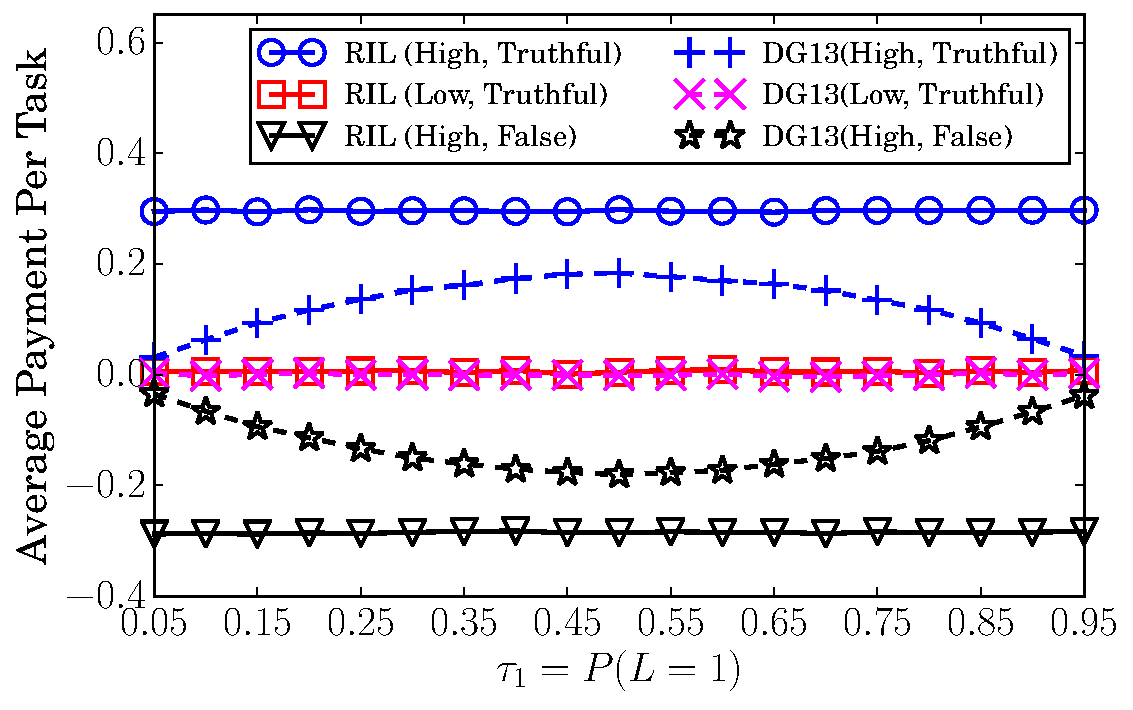
\includegraphics[width=\textwidth]{image/BPP1}
        \caption{\label{BIM2}}
    \end{subfigure}%
    ~
    \begin{subfigure}[t]{0.32\textwidth}
        \centering
        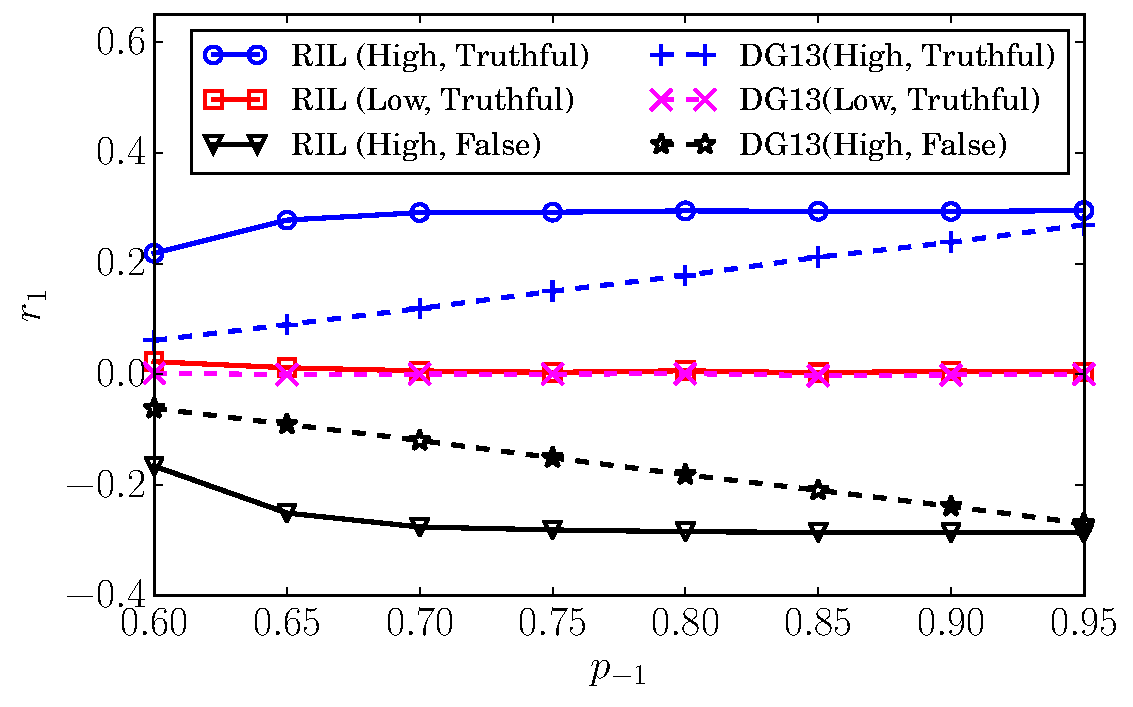
\includegraphics[width=\textwidth]{image/BPP2}
        \caption{\label{BIM3}}
    \end{subfigure}
        ~
    \begin{subfigure}[t]{0.32\textwidth}
        \centering
        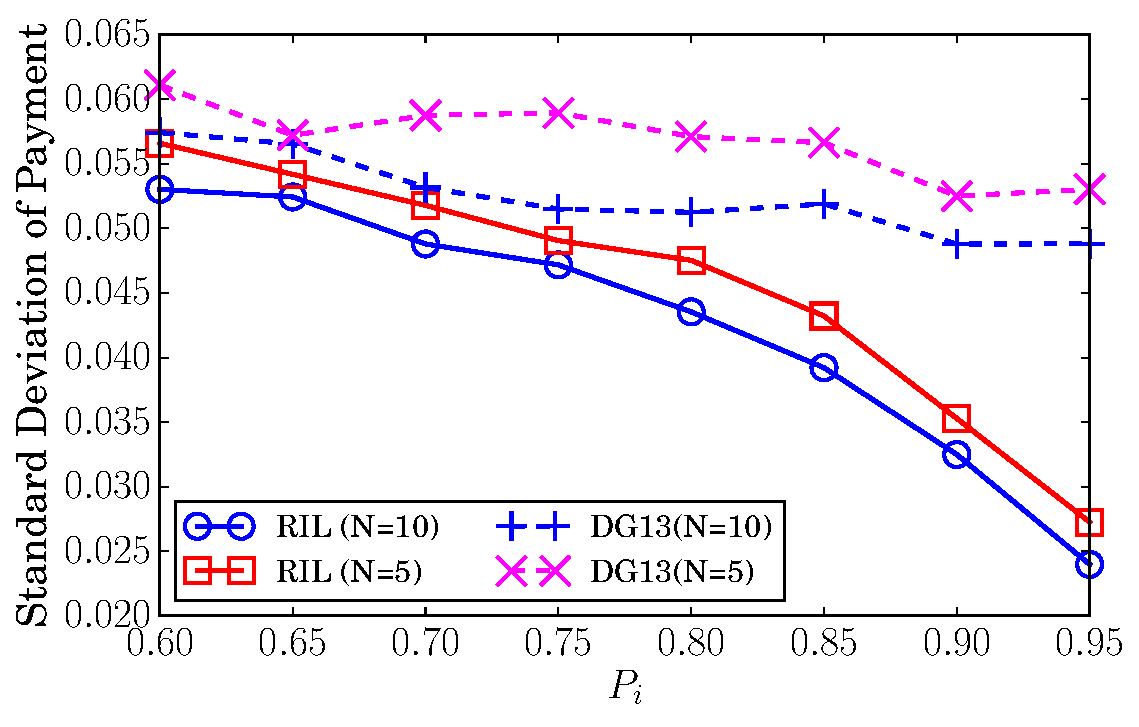
\includegraphics[width=\textwidth]{image/BPP3}
        \caption{\label{BIM4}}
    \end{subfigure}
%	~
%	\begin{subfigure}[t]{0.24\textwidth}
%        \centering
%        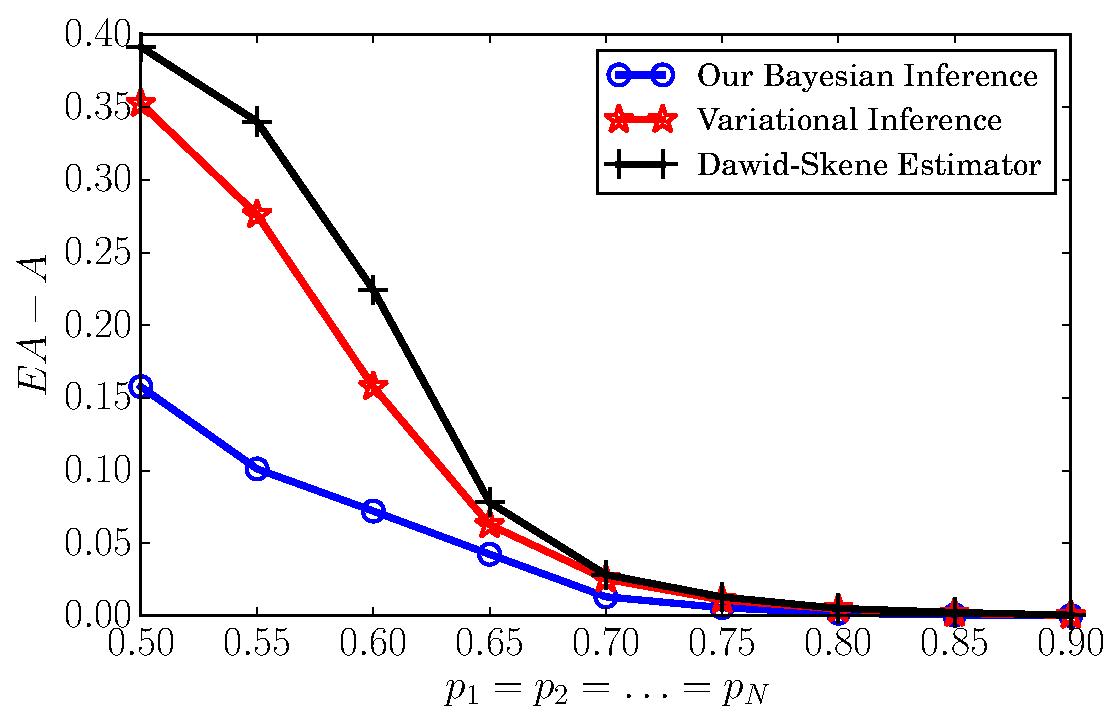
\includegraphics[width=\textwidth]{image/EXPC1}
%        \caption{\label{BIM1}}
%    \end{subfigure}
    \caption{\label{BIM} Empirical analysis on our Bayesian inference algorithm. (a) Average payment per task given true label's distribution. (b) Average payment per task given PoBCs of workers excluding $i$. (c) The standard deviation of the payment given worker $i$'s PoBC.}
\vspace{-2mm}
\end{figure*}
\subsection{Proof for Long-Term IC}
Due to the one-step IC in our mechanism, we know that, to get higher long-term payments, worker $i$ must mislead our RL algorithm into at least increasing the scaling factor from $a$ to any $a'>a$ at a certain state $s$.
Actually, our RL algorithm will only increase the scaling factor when the state-action value function satisfies $Q^{\pi}(s,a)\leq Q^{\pi}(s,a')$.
Eqn.\ref{equation:approx_reward} tells us that our objective function consists of the utility obtained from the collected labels ($F(\tilde{A}^t)$) and the utility lost in the payment ($\eta {\sum}_{i=1}^{N}P^t_i$).
Once we increase the scaling factor, we at least need to increase the payments for the other $N-1$ workers by $M(N-1)\mathbb{P}_H\cdot G_{\mathcal{A}}$, which corresponds to the left-hand side of Eqn.\ref{Condition}.

On the other hand, for the obtained utility, we can have 
\begin{lemma}
\label{ConvBoundxx}
In any time step $t$, if all workers except for worker $i$ report truthfully and exert high efforts,
\begin{equation*}
F(\tilde{A}^t)\leq F(1) \;\;,\; F(\tilde{A}^t)\geq F(1-\psi)
\end{equation*}
where $\psi$ is defined in Eqn.\ref{equation:psi}.
\end{lemma}
We again defer the detailed proof to the supplementary material.
Our main idea is to derive the bounds of $\tilde{A}$ by analyzing the distribution of $\tilde{\sigma}_j$.
Our motivation comes form Eqn.\ref{vot} which ensures, $\tilde{A} \approx 1-\mathbb{E}[1/(1+e^{|\tilde{\sigma}_j|})]$. From Lemma~\ref{ConvBoundxx}, we can know that, even in the long-term, worker $i$ can at most increase our value by $(1-\gamma)^{-1}[F(1)-F(1-\psi)]$, which corresponds to the right-hand side of Eqn.\ref{Condition}.

Thereby, if Eqn.\ref{Condition} is satisfied, worker $i$ will be unable to make up our value loss increment in the payments, and our RL algorithm will reject the hypothesis to increase the scaling factor.
In this case, the only payment-maximizing strategy for worker $i$ is to report truthfully and exert high efforts in all time steps, which concludes Theorem~\ref{RMNE}.

%Taking our analysis about the payment increment at the beginning of this section, worker $i$'s deviation will not be suffice to change the objective value function's optimal solution to a higher scaling factor if Eqn.\ref{Condition} is satisfied - the increase in accuracy is less than the additional payment.
%In this case, our RL algorithm will not respond to the strategy changes of worker $i$, which concludes Theorem~\ref{RMNE}.
%
%
%
%If worker $i$ cannot make up our value loss increment in the payments, our RL algorithm will reject the hypothesis to increase the scaling factor, and the only payment-maximizing strategy for worker $i$ is to report truthfully and exert high efforts in all time steps.
%Thus, our proof will focus on the right-hand side of Eqn.\ref{Condition} which denotes the upper bound of the value increment that worker $i$ can bring.
%
%Following our analysis in the beginning of this section, to prove Theorem~\ref{RMNE}, we need to derive the upper bound of the value increment that worker $i$ can bring.
%Worker $i$ can only increase our value by increasing the estimated label accuracy $\tilde{A}$.
%From Eqn.\ref{vot}, we can know that, when $M\gg 1$, the estimated accuracy $\tilde{A}$ satisfies
%\begin{equation}
%\label{accP}
%\tilde{A} \approx 1-\mathbb{E}g(\tilde{\sigma}_j)\;\;,\;\; g(\tilde{\sigma}_j)=1/(1+e^{|\tilde{\sigma}_j|}).
%\end{equation}
%From the proof of Theorem~\ref{OSEqulibrium}, we can know that $\tilde{\mathbb{P}}^{t}_i \approx \mathbb{P}^{t}_i$.
%In this case, according to Eqn.\ref{ProbRatio}, we can have
%\begin{equation}
%\label{ProbRatioApp}
%\tilde{\sigma}_j(\mathbb{P}_i)\approx \log\left(\frac{\tau_{1}}{\tau_{2}}\lambda_i^{\delta_{ij1}-\delta_{ij2}}{\prod}_{k\neq i}\lambda_H^{\delta_{kj1}-\delta_{kj2}}\right).
%\end{equation}
%where $\lambda_i=\mathbb{P}_i/(1-\mathbb{P}_i)$ and $\lambda_H=\mathbb{P}_H/(1-\mathbb{P}_H)$.
%%In this proof, if the superscripts of variables in an equation are not specified, the equation should hold for any time step $t$. Suppose all workers except worker $i$ report truthfully and exert high efforts at all time steps.
%%Then, at step $t$, according to Proposition~\ref{ConvBound}, under the condition of Proposition~\ref{OSEqulibrium}, 
%%both $\mathbb{E}[m/M]$ and $\mathbb{E}[m/M]^2$ approaches $0$.
%%In this case, $\tilde{p}_i\rightarrow p_i$. Thus, the log-ratio, which is used for computing the posterior accuracy in Equation~\ref{vot} satisfies
%%\begin{equation}
%%\label{ProbRatioApp}
%%\tilde{\sigma}_j(p_i)\approx \log\left(\frac{\tau_{1}}{\tau_{2}}\lambda_i^{\delta_{ij1}-\delta_{ij2}}{\prod}_{k\neq i}\lambda_H^{\delta_{kj1}-\delta_{kj2}}\right).
%%\end{equation}
%
%We know that $\tilde{A}\leq 1.0$ holds no matter what strategy worker $i$ takes. Thus, to bound the value increment caused by worker $i$'s strategy changes, we consider two cases where worker $i$ intentionally provides low-quality labels:
%
%\underline{\textbf{Case 1}:} If $\mathbb{P}_i=0.5$, we can eliminate $\lambda_i$ from Eqn.\ref{ProbRatioApp} because $\lambda_i=1$. Furthermore, according to Lemma~\ref{Su-Concave2} in the supplementary file, we can know that 
%$g(\tilde{\sigma}_j)< e^{\tilde{\sigma}_j}$ and $g(\tilde{\sigma}_j)< e^{-\tilde{\sigma}_j}$ both hold. Thus, we build a tighter upper bound of $g(\tilde{\sigma}_j)$ by dividing all the combinations of $\delta_{kj1}$ and $\delta_{kj2}$ in Eqn.\ref{ProbRatioApp} into two sets and using the smaller one of $e^{\tilde{\sigma}_j}$ and $e^{-\tilde{\sigma}_j}$ in each set.
%By using this method, if the true label is $1$, we can have $\mathbb{E}_{[L(j)=1]}g(\tilde{\sigma}_j)< q_1+q_2$, where
%\begin{equation*}
%\begin{split}
%&q_1 = \frac{\tau_2}{\tau_1}{\sum}_{n=K+1}^{N-1}C_{N-1}^{n} (\frac{1}{\lambda_H})^{n-m}\mathbb{P}_H^n(1-\mathbb{P}_H)^m\\
%&q_2 = \frac{\tau_1}{\tau_2}{\sum}_{n=0}^{K}C_{N-1}^{n} {\lambda_H}^{n-m}\mathbb{P}_H^n(1-\mathbb{P}_H)^m\\
%&n={\sum}_{k\neq i}\delta_{kj1}\;,\;m= {\sum}_{k\neq i}\delta_{kj2}
%\end{split}
%\end{equation*}
%and $K=\lfloor (N-1)/2 \rfloor$. By using Lemma~\ref{Su-Concave3} in the supplementary file, we can thus get
%\begin{equation*}
%\begin{split}
%\mathbb{E}_{[L(j)=1]}g(\tilde{\sigma}_j) < c_{\tau}[4\mathbb{P}_H(1-\mathbb{P}_H)]^{\frac{N-1}{2}}.
%\end{split}
%\end{equation*}
%where $c_{\tau}=\tau_1\tau_2^{-1}+\tau_1^{-1}\tau_2$. Similarly,
%\begin{equation*}
%\begin{split}
%\mathbb{E}_{[L(j)=2]}g(\tilde{\sigma}_j) < c_{\tau}[4\mathbb{P}_H(1-\mathbb{P}_H)]^{\frac{N-1}{2}}.
%\end{split}
%\end{equation*}
%Thereby, $\tilde{A}>1-c_{\tau}[4\mathbb{P}_H(1-\mathbb{P}_H)]^{\frac{N-1}{2}}=1-\psi$.
%
%
%\underline{\textbf{Case 2}:} If $\mathbb{P}_i=1-\mathbb{P}_H$, we can rewrite Eqn.\ref{ProbRatioApp} as
%\begin{equation*}
%\tilde{\sigma}_j(1-\mathbb{P}_H)\approx \log\left(\frac{\tau_{1}}{\tau_{2}}\lambda_H^{x-y}{\prod}_{k\neq i}\lambda_H^{\delta_{kj1}-\delta_{kj2}}\right)
%\end{equation*}
%where $x=\delta_{ij2}$ and $y=\delta_{ij1}$. Since $\mathbb{P}_i=1-\mathbb{P}_H$, $x$ and $y$ actually has the same distribution as $\delta_{kj1}$ and $\delta_{kj2}$. Thus, the distribution of $\tilde{\sigma}_j(1-\mathbb{P}_H)$ is actually the same as $\tilde{\sigma}_j(\mathbb{P}_H)$.
%In other words, since Proposition~\ref{OSEqulibrium} ensures $\tilde{\mathbb{P}}_i\approx\mathbb{P}_i$, our Bayesian inference algorithm uses the information provided by worker $i$ via flipping the label when $\mathbb{P}_i<0.5$.
%%\end{itemize}
%
%
%Thus, even if worker $i$ intentionally lowers the label quality, $\tilde{A}\geq 1-\psi$ still holds.
%Considering $F(\cdot)$ is a non-decreasing monotonic function, we know that worker $i$ can at most increase data requester's objective function by $F(1)-F(1-\psi)$ in each step and $(1-\gamma)^{-1}[F(1)-F(1-\psi)]$ in the long-term.
%Taking our analysis about the payment increment at the beginning of this section, worker $i$'s deviation will not be suffice to change the objective value function's optimal solution to a higher scaling factor if Eqn.\ref{Condition} is satisfied - the increase in accuracy is less than the additional payment.
%In this case, our RL algorithm will not respond to the strategy changes of worker $i$, which concludes Theorem~\ref{RMNE}.



%Considering the case that worker $i$ exert low efforts and reports randomly, namely $p_i=0.5$, we can eliminate $\lambda_i$ from Equation~\ref{ProbRatioApp} because $\lambda_i=1$.
%Furthermore, according to Lemma~\ref{Su-Concave2} in the supplementary file, we can know that 
%$g(\tilde{\sigma}_j)< e^{\tilde{\sigma}_j}$ and $g(\tilde{\sigma}_j)< e^{-\tilde{\sigma}_j}$ both hold.
%Thus, we build a more tight upper bound of $g(\tilde{\sigma}_j)$ by dividing all the combinations of $\delta_{kj1}$ and $\delta_{kj2}$ in Equation~\ref{ProbRatioApp} into two sets and using the smaller one of $e^{\tilde{\sigma}_j}$ and $e^{-\tilde{\sigma}_j}$ in each set.
%By using this method, if the true label is $1$, we can have $\mathbb{E}_{[L(j)=1]}g(\tilde{\sigma}_j)< q_1+q_2$, where
%\begin{equation*}
%\begin{split}
%&q_1 = \frac{\tau_2}{\tau_1}{\sum}_{n=K+1}^{N-1}C_{N-1}^{n} (\frac{1}{\lambda_H})^{n-m}p_H^n(1-p_H)^m\\
%&q_2 = \frac{\tau_1}{\tau_2}{\sum}_{n=0}^{K}C_{N-1}^{n} {\lambda_H}^{n-m}p_H^n(1-p_H)^m\\
%&n={\sum}_{k\neq i}\delta_{kj1}\;,\;m= {\sum}_{k\neq i}\delta_{kj2}\;,\;K=\lfloor (N-1)/2 \rfloor.
%\end{split}
%\end{equation*}
%Here, we use $e^{-\tilde{\sigma}_j}$ and $e^{\tilde{\sigma}_j}$ as the upper bound of $g(\tilde{\sigma}_j)$ when $n\in (K, N-1]$ and $n\in [0, K]$, respectively. By using Lemma~\ref{Su-Concave3} in the supplementary file, we can thus get
%\begin{equation}
%\begin{split}
%\mathbb{E}_{[L(j)=1]}g(\tilde{\sigma}_j) < c_{\tau}[4p_H(1-p_H)]^{\frac{N-1}{2}}.
%\end{split}
%\end{equation}
%where $c_{\tau}=\tau_1\tau_2^{-1}+\tau_1^{-1}\tau_2$. Similarly,
%\begin{equation}
%\begin{split}
%\mathbb{E}_{[L(j)=2]}g(\tilde{\sigma}_j) < c_{\tau}[4p_H(1-p_H)]^{\frac{N-1}{2}}.
%\end{split}
%\end{equation}
%Thereby, $\tilde{A}>1-2c_{\tau}[4p_H(1-p_H)]^{\frac{N-1}{2}}=1-\psi$.


%We then consider another case where worker $i$ exerts high efforts but reports falsely, namely $p_i=1-p_H$. In this case, we can rewrite Equation~\ref{ProbRatioApp} as
%\begin{equation}
%\tilde{\sigma}_j(1-p_H)\approx \log\left(\frac{\tau_{1}}{\tau_{2}}\lambda_H^{x-y}{\prod}_{k\neq i}\lambda_H^{\delta_{kj1}-\delta_{kj2}}\right).
%\end{equation}
%where $x=\delta_{ij2}$ and $y=\delta_{ij1}$. Since $p_i=1-p_H$, $x$ and $y$ actually has the same distribution as $\delta_{kj1}$ and $\delta_{kj2}$. Thus, the distribution of $\tilde{\sigma}_j(1-p_H)$ is actually the same as $\tilde{\sigma}_j(p_H)$.
%In other words, since Proposition~\ref{OSEqulibrium} ensures $p_i$ to be accurately estimated, our Bayesian inference algorithm uses the information provided by worker $i$ via flipping the label when $p_i<0.5$.
%Thus, $p_i=0.5$ actually lowers $\tilde{A}$ to the utmost because worker $i$ provides no information about the true label in this case.
%Thus, $\tilde{A}\geq 1-\psi$ always holds.
%On the other hand, $\tilde{A}\leq 1.0$ also always holds.
%Considering $F(\cdot)$ is a non-decreasing monotonic function, we can get $X(a)\geq (1-\rho)^{-1}F(1-\psi)$ while $X(b) \leq (1-\rho)^{-1}F(1)$.
%Thereby, when Equation~\ref{Condition} is satisfied, $X(a)-X(b)+Y>0$ always holds, which concludes Proposition~\ref{RMNE}.